% Lecture Template for ME3023 -  Measurements in Mechanical Systems - Tennessee Technological University
% Spring 2020 - Summer 2020 - Fall 2020 - Spring 2021 - Summer 2021 - Fall 2023
% Tristan Hill, May 07, 2020 - June 12, 2020 - July 08, 2020 - Novemeber 02, 2020 - March 28, 2021 - May 25, 2021 - August 21, 2022 - September 02, 2023 - September 09, 2023

% Fall 2023 - condensing and streamlining lectures by combining topics into a single PDF under the module name
%			  this will simplify file and link management as well as make lectures easier to use in class
%			- added image/ to clean directory and reduce redundancy, specific to module for now  

% Module Name: - Steady State Circuits
% Topic 1 - Components, Units, and Symbols
% Topic 2 - Fundamental Laws
% Topic 3 - Circuit Applications


\documentclass[fleqn]{beamer} % for presentation (has nav buttons at bottom)
\usepackage{../measurements_lectures}

\author{ME3023 - Measurements in Mechanical Systems} % original formatting from Mike Renfro, September 21, 2004

\newcommand{\MNUM}{4\hspace{2mm}} % module number 
\newcommand{\moduletitle}{Steady State Circuits}

\newcommand{\sectionItitle}{Components, Units, and Symbols}
\newcommand{\sectionIItitle}{Fundamental Laws}
\newcommand{\sectionIIItitle}{Circuit Applications}

\newcommand{\sectionIsubsectionItitle}{Passive Components}
\newcommand{\sectionIsubsectionIItitle}{Electrical Quantities}
\newcommand{\sectionIsubsectionIIItitle}{Units and Symbols}
\newcommand{\sectionIsubsectionIVtitle}{Types of Switches}

\newcommand{\sectionIIsubsectionItitle}{Ohm's Law}
\newcommand{\sectionIIsubsectionIItitle}{Combining Resistance}
\newcommand{\sectionIIsubsectionIIItitle}{Kirchhoff's Laws}
\newcommand{\sectionIIsubsectionIVtitle}{Power Dissipation}

\newcommand{\sectionIIIsubsectionItitle}{Circuits in Mechanical Engineering}
\newcommand{\sectionIIIsubsectionIItitle}{Drain Pipe Theory}
\newcommand{\sectionIIIsubsectionIIItitle}{Example 1: LED Circuit}
\newcommand{\sectionIIIsubsectionIVtitle}{Example 2: LDR circuit}

% custom box
\newsavebox{\mybox}

\title{Lecture Module - \moduletitle}

\date{Mechanical Engineering\vspc Tennessee Technological University}

\begin{document}

	\lstset{language=MATLAB,basicstyle=\ttfamily\small,showstringspaces=false}

	\frame{\titlepage \center\begin{framed}\Large \textbf{Module \MNUM - \moduletitle}\end{framed} \vspace{5mm}}

	% Module Outline
	\begin{frame} 
		\large \textbf{Module \MNUM - \moduletitle} \vspace{3mm}\\

		\begin{itemize}
			\item Topic 1 - \hyperlink{sectionI}{\sectionItitle} \vspc % section I
			\item Topic 2 - \hyperlink{sectionII}{\sectionIItitle} \vspc % section II
			\item Topic 3 - \hyperlink{sectionIII}{\sectionIIItitle} \vspc % section III
		\end{itemize}

	\end{frame}

	% section I
	\section{\sectionItitle}\label{sectionI}

		% section I Outline
		\begin{frame} 
			\large \textbf{Topic 1 - \sectionItitle} \vspace{3mm}\\

			\begin{itemize}
				\item \hyperlink{sectionIsubsectionI}{\sectionIsubsectionItitle} \vspc %  section I subsection I
				\item \hyperlink{sectionIsubsectionII}{\sectionIsubsectionIItitle} \vspc % section I subsection II
				\item \hyperlink{sectionIsubsectionIII}{\sectionIsubsectionIIItitle} \vspc % section I subsection III
				\item \hyperlink{sectionIsubsectionIV}{\sectionIsubsectionIVtitle} \vspc % section I subsection IV
			\end{itemize}
		\end{frame}
		
		% section I subsection I 
		\subsection{\sectionIsubsectionItitle}\label{sectionIsubsectionI}

			\begin{frame}
				\frametitle{\sectionIsubsectionItitle}
				
				Passive components affect the behavior of a circuit in different ways but they do   not generate power and can only absorb energy or transform it into heat. Active components on the other hand...

				\begin{itemize}
				\item 
				\item
				\item
				\end{itemize}

				Most circuits require an active power source for operation. A voltage source is used in most applications however current sources are also available and are needed for specialized electrical applications. 

			\end{frame}

			\begin{frame}
				\frametitle{\sectionIsubsectionItitle}

				Components are identified by color codes and numbering systems. However it is always a good idea to measure for yourself because a marking can be  incorrect  or a component may be damaged. \vspc

				\includegraphics[scale=.25]{images/resistor_color_codes.jpg}
				\includegraphics[scale=.3]{images/ceramic_capacitor_codes.jpg}

			\end{frame}

		% section I subsection II
		\subsection{\sectionIsubsectionIItitle}\label{sectionIsubsectionII}

			\begin{frame}
				\frametitle{\sectionIsubsectionIItitle}

				\begin{itemize}

					\begin{multicols}{2}
					\item {\BL\underline{\hspace{30mm}}} - the physical property of matter that causes it to experience a force when placed in an electromagnetic field.
					
					\includegraphics[scale=.5]{images/charges_plus_minus.png}
					\end{multicols}
					
					\item {\PR \BL\underline{\hspace{30mm}}} - the difference in electric potential between two points ... can be caused by electric charge, by electric current through a magnetic field, by time-varying magnetic fields, or some combination of these three.
					
					\item {\RD \BL\underline{\hspace{30mm}}} - the rate of flow of electric charge past a point or region. An electric current is said to exist when there is a net flow of electric charge through a region.

				\end{itemize}	

			\end{frame}

			\begin{frame}
				\frametitle{\sectionIsubsectionIItitle}
				
				\begin{itemize}

					\item {\BL \BL\underline{\hspace{30mm}}} - a measure of a components opposition to the flow of electric current. The inverse quantity is electrical conductance, and is the ease with which an electric current passes.  
							
					\item {\PR \BL\underline{\hspace{30mm}}} - the ratio of the change in electric charge of a system to the corresponding change in its electric potential (voltage).
					
					\item {\RD \BL\underline{\hspace{30mm}}} - the tendency of an electrical conductor to oppose a change in the electric current flowing through it. The flow of electric current creates a magnetic field around the conductor. The field strength depends on the magnitude of the current, and follows any changes in current.

				\end{itemize}

			\end{frame}


		% section I subsection III
		\subsection{\sectionIsubsectionIIItitle}\label{sectionIsubsectionIII}
			\begin{frame} 
				\frametitle{\sectionIsubsectionIIItitle}

				\renewcommand{\arraystretch}{1.2}
				\begin{tabular}{|c|c|c|c|} \hline
					Quantity & Symbol & Unit & Abbr. \\ \hline\hline
				    Charge & Q,q & Coulomb & C \\ \hline
				    Voltage & V,v & Volt & v\\ \hline
				    Current & I,i & Ampere & A \\ \hline
				    Resistance & R & Ohm & $\Omega$ \\ \hline
				    Capacitance & C & Farad & F \\ \hline
				    Inductance & L & Henry & H  \\ \hline
				\end{tabular}
				
				\vspace*{10mm} Question: When should you use upper case or lower case letters for electrical quantities?
				
			\end{frame}	

			\begin{frame} 
				\frametitle{\sectionIsubsectionIIItitle}

				When working with a or building a circuit  you need a diagram. Draw or find one before you begin. Here are some commonly used symbols.\vspccc

				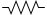
\includegraphics[scale=.4]{images/resistor_symbol.png} \hspace{15mm}
				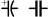
\includegraphics[scale=.4]{images/capacitor_symbol.png} \hspace{15mm}
				\includegraphics[scale=.4]{images/inductor_symbol.png} \vspace{10mm}
				
				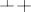
\includegraphics[scale=.5]{images/node_symbol.png} \hspace{15mm}
				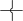
\includegraphics[scale=.5]{images/jump_symbol.png} \hspace{15mm}
				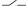
\includegraphics[scale=.5]{images/switch_symbol.png} \hspace{15mm}
				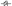
\includegraphics[scale=.7]{images/led_symbol.png} \hspace{15mm}
				
			\end{frame}	

		% section I subsection IV
		\subsection{\sectionIsubsectionIVtitle}\label{sectionIsubsectionIV}	

			\begin{frame}
				\frametitle{\sectionIsubsectionIVtitle}

				A switch is a mechanical-electrical device that that can change from a continuous state to a dis-continuous state and they are used as a mechanical interface to a circuit. There many different types of switches for different purposes and this is not an exhaustive list.

				\begin{itemize}
				\item Toggle Switches
				\item Momentary Switches
				\item Reed Switches
				\item Level or Float Switches
				\item and many more
				\end{itemize}
				
			\end{frame}

			\begin{frame}
				\frametitle{\sectionIsubsectionIVtitle}
				
				\small

				Toggle switches are are possibly the most commonly used switches and they come in many different forms.\vspace{5mm}\\

				{\bf Poles } - The numbers of poles refers to the number of independent conductors or circuits in a switch that are controlled by the same toggle or input.
				
				{\bf Throws} - The numbers of throws refers to the number of output terminals of a switch per pole. \vspace{5mm}\\
				
				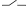
\includegraphics[scale=.7]{images/spst_symbol.png} \hspace{5mm} 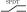
\includegraphics[scale=.7]{images/spdt_symbol.png} \hspace{5mm}
				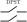
\includegraphics[scale=.7]{images/dpst_symbol.png} \hspace{5mm} 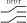
\includegraphics[scale=.7]{images/dpdt_symbol.png}

			\end{frame}

	
	% Section II
	\section{\sectionIItitle}\label{sectionII}

		% section II Outline
		\begin{frame}
			\large \textbf{Topic 2 - \sectionIItitle} \vspace{3mm}\\

			\begin{itemize}
				\item \hyperlink{sectionIIsubsectionI}{\sectionIIsubsectionItitle} \vspc %  section II subsection I
				\item \hyperlink{sectionIIsubsectionII}{\sectionIIsubsectionIItitle} \vspc % section II subsection II
				\item \hyperlink{sectionIIsubsectionIII}{\sectionIIsubsectionIIItitle} \vspc % section II subsection III
				\item \hyperlink{sectionIIsubsectionIV}{\sectionIIsubsectionIVtitle} \vspc % section II subsection IV
			\end{itemize}

		\end{frame}

		% section II subsection I
		\subsection{\sectionIIsubsectionItitle}\label{sectionIIsubsectionI}

			\begin{frame}[label=sectionIIsubsectionI]
				\frametitle{\sectionIIsubsectionItitle}

				\begin{multicols}{3}

					{\bf James Maxwell}
					\includegraphics[scale=.30]{images/James_Clerk_Maxwell.png} \hspace{3mm}	

					{\bf George Ohm} 
					\includegraphics[scale=.30]{images/George_Ohm.png}	

					{\bf Ohm's Notebook}
					\includegraphics[scale=.07]{images/Ohms_Laborbuch.jpg}	

				\end{multicols}
				Ohm did his work on resistance in the years 1825 and 1826, and published his results in 1827 as the book Die galvanische Kette, mathematisch bearbeitet...

			\end{frame}

		    \begin{frame}[label=sectionIIsubsectionI]
				\frametitle{\sectionIIsubsectionItitle}


				Ohm's law states that the current through a conductor between two points is directly proportional to the voltage across the two points. 

				\begin{multicols}{2}

					\[ I=\frac{V}{R}  \] \vspace{1mm}\\
					It is more commonly shown in the following form.
					\[ V=IR \]

					\includegraphics[scale=.8]{images/OhmsLaw.png}

				\end{multicols}

			\end{frame}	

		% section II subsection II
		\subsection{\sectionIIsubsectionIItitle}\label{sectionIIsubsectionII}

			\begin{frame}
				\frametitle{\sectionIIsubsectionIItitle}

				\begin{multicols}{2}

					\begin{center}
					Resistors in Series\vspcc
					\includegraphics[scale=.2]{images/series_resistors.png} 
					\end{center}
					\[R_{eq}=R_1+R_2 \]
					\vspace{15mm}\\

					\begin{center}
					Resistors in Parallel \vspcc
					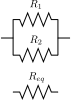
\includegraphics[scale=.2]{images/parallel_resistors.png}
					\end{center}
					\[R_{eq}=\frac{1}{\frac{1}{R_1}+\frac{1}{R_2}} \]
					\vspace{10mm}\\

				\end{multicols}

			\end{frame}

		% section II subsection III
		\subsection{\sectionIIsubsectionIIItitle}\label{sectionIIsubsectionIII}

			\begin{frame}
				\frametitle{\sectionIIsubsectionIIItitle}

				Both of Kirchhoff's laws can be understood as corollaries of Maxwell's equations in the low-frequency limit. They are accurate for DC circuits, and for AC circuits at frequencies where the wavelengths of electromagnetic radiation are very large compared to the circuits. \vspc 

				\begin{enumerate}
				\item Kichhoff's Voltage Law (KVL)
				\item Kichhoff's Current  Law (KCL)
				\end{enumerate}

			\end{frame}

			\begin{frame}
				\frametitle{\sectionIIsubsectionIIItitle}

				\begin{multicols}{2}
					{\bf Kichhoff's Voltage Law (KVL)} - The sum of the voltages around a loop (aka mesh) equals zero.\\ $ \sum\limits_{k=1}^{n} v_k = 0 $ \\
					\includegraphics[scale=.20]{images/Kirchhoffs_voltage_law.png} 

					{\bf Kichhoff's Current  Law (KCL)} - The sum of the current flowing in and out of  node (aka junction) equals zero. \\ $ \sum\limits_{k=1}^{n} i_k = 0 $ \vspace{2mm}\\
					\includegraphics[scale=.4]{images/Kirchhoffs_current_law.png} 
				\end{multicols}

			\end{frame}

			\begin{frame}
			\frametitle{\sectionIIsubsectionIIItitle}


			\end{frame}

		% section II subsection IV 
		\subsection{\sectionIIsubsectionIVtitle}\label{sectionIIsubsectionIV}

			\begin{frame}
				\frametitle{\sectionIIsubsectionIVtitle}

				Energy is transformed in to heat in passive circuit components. For a resistor the power dissipation can be found with following relations. \vspace{5mm}
	
				\[P=IV \hspace{20mm} V=IR \]

			\end{frame}

			\begin{frame}
				\frametitle{\sectionIIsubsectionIVtitle}

				Power is the rate of energy dissipated, aka the amount of energy lost per unit of time. How do we compute total energy for the power? 
	
				\[E=\int\limits_{t1}^{t2}Pdt \]  

			\end{frame}
		
	% Section III
	\section{\sectionIIItitle}\label{sectionIII}

		% section III Outline
		\begin{frame}
			\large \textbf{Topic 3 - \sectionIIItitle} \vspace{3mm}\\

			\begin{itemize}
				\item \hyperlink{sectionIIIsubsectionI}{\sectionIIIsubsectionItitle} \vspc %  section III subsection I
				\item \hyperlink{sectionIIIsubsectionII}{\sectionIIIsubsectionIItitle} \vspc % section III subsection II
				\item \hyperlink{sectionIIIsubsectionIII}{\sectionIIIsubsectionIIItitle} \vspc % section III subsection III
				\item \hyperlink{sectionIIIsubsectionIV}{\sectionIIIsubsectionIVtitle} \vspc % section III subsection IV
			\end{itemize}

		\end{frame}

		% section III subsection I
		\subsection{\sectionIIIsubsectionItitle}\label{sectionIIIsubsectionI}

			\begin{frame}
				\frametitle{\sectionIIIsubsectionItitle}

				How much does a mechanical engineer need to know about electricity and magnetism? This is good question, and obviously it varies based on your particular area of mechanical engineering. However...
	
				\begin{itemize}
					
					\item System design is integrated! Look around you, can you find anything that was developed or designed without circuits? Engineering is an integrated discipline and very few products or designs are isolated so to a single field.
					
					\item Further, the need for measurements in mechanical systems drives the need for a mechanical engineer to have a solid foundation in basic circuits theory.
						
				\end{itemize}

				
			\end{frame}

			\begin{frame}
				\frametitle{\sectionIIIsubsectionItitle}
				
				{\bf Mechatronics} \\
				Many devices or designs combine mechanical and electrical systems. This is known as Mechatronics and if you are interested in this area you are in a great place to learn. TnTech Mechanical Engineering offers a concentration in Mechatronics Engineering. In this degree you will study both mechanical engineering and electrical engineering topic to give you the foundation to design truly integrated systems! Ask me or Dr. Canfield if you have any questions about this. 

			\end{frame}

		% section III subsection II
		\subsection{\sectionIIIsubsectionIItitle}\label{sectionIIIsubsectionII}	

			\begin{frame}
				\frametitle{\sectionIIIsubsectionIItitle}

				{\bf Fluid Flow - Hydraulic Analogy} \vspc
	
				Traditionally engineers have used an analogy relating the movement of electrons to the flow of water through a pipe (\href{https://en.wikipedia.org/wiki/Hydraulic_analogy}{\BL hydraulic analogy}) known as {\it drain-pipe theory}. \vspace{5mm}
				
				This may provide a sense of intuition {\it however} this comparison is not accurate do to the non-Newtonian nature of electricity and magnetism (\href{https://www.slideshare.net/PDiCEOThaneHeins3240/georgia-state-university-hyperphysics-how-newtonian-mechanics-is-incorrectly-being-applied-to-explain-the-laws-of-electricity-and-magnetism}{\GR more on this}). It can  be used to visualize some basic circuits principles, but it should not be used for analysis of complex electrical systems. 

			\end{frame}

		% section III subsection III
		\subsection{\sectionIIIsubsectionIItitle}\label{sectionIIIsubsectionIII}

			\begin{frame}
				\frametitle{\sectionIIIsubsectionIIItitle}

				LEDs or Light Emitting Diodes are used more and more everyday and traditional {\it incandescent} lights are used rarely in new deigns.\\
				Why are LEDs better? Can you think of any trade-offs? \\

				\begin{multicols}{2}
					Pros:
					\begin{itemize}
						\item 
						\item
						\item
					\end{itemize}
					Cons:
					\begin{itemize}
						\item 
						\item
						\item
					\end{itemize}
				\end{multicols}

			\end{frame}

			\begin{frame}
				\frametitle{\sectionIIIsubsectionIIItitle}

				Design a circuit with a voltage source, an LED, a resistor, and a SPST switch for turning on the LED. Choose the resistor such that the current is in the appropriate for a typical LED ($\sim 20mA$). The voltage drop for a green LED at $\sim 20mA$ in known to be $\sim 3.5 v$. \vspace{30mm}

			\end{frame}

		% section III subsection IV
		\subsection{\sectionIIIsubsectionIVtitle}\label{sectionIIIsubsectionIV}	

			\begin{frame}
				\frametitle{\sectionIIIsubsectionIVtitle}

				\small

				Consider this circuit for measuring light intensity with an LDR (light dependent resistor). The sensors is used in a voltage divider circuit. 

				\begin{multicols}{2}
					\includegraphics[scale=.20]{images/ldr_circuit.png}

					\begin{enumerate}

						\item Find the current in the circuit.
						\item Find the voltage across the LDR and the $10K\Omega$ resistor.
						\item Find the total energy dissipated in the circuit over 60 seconds.\vspc

						\item Question: Why is the $10K\Omega$ resistor needed? 

					\end{enumerate}
				\end{multicols}

			\end{frame}

			\begin{frame}
				\frametitle{\sectionIIIsubsectionIVtitle}
				Space to work


			\end{frame}

\end{document}





